\scanpage{91}
\mspage{90}
\mspage{43}

supposer $X$ affine et qu'il existe un préschéma affine $X'_1$, de présentation finie, quasi fini et fidèlement plat sur $X$, et un $X$-morphisme $X'_1\longrightarrow X'$, ce qui nous ramène au cas où $f$ est quasi-fini. Quitte à localiser encore sur $X$, au sens de la topologie étale cette fois, on voit qu'il existera un ouvert $X'_1$ de $X'$ tel que $X'_1\longrightarrow X$ soit fini et surjectif, ce qui nous ramène au cas où $f$ est fini et surjectif, déjà traité dans a).

9.4.4. Dans le cas d), on peut supposer (en se localisant sur $X$) que $X$ est réduit à un seul point, et même contenu de 1.1. \unsure{qr'il|qu'il} est spectre d'un corps $k$, puis (quitte à remplacer $X'$ par un ouvert affine non vide) que $X'$ est affine et à fortiori $f$ est quasi compact et quasi séparé. Mais alors il est encore vrai que $f_*$ commute à tout changement de base $Y\longrightarrow X$, comme nous verrons ultérieurement. De plus, $f$ est universellement ouvert (EGA IV 2.4.9.) donc on est sous les conditions de 9.1., et le raisonnement de 9.4.1. s'applique encore.

\margin{\figure{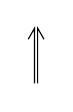
\begin{tikzpicture}\draw (0,0)--(0,0.7)--(-0.08,0.56);\draw (0.04,0)--(0.04,0.7)--(0.12,0.56);\end{tikzpicture}}}

\inserted{Ceci achève la démonstration de 9.4.}
